\chapter{池化层}

池化层是当前卷积神经网络中常用组件之一,它最早见于LeNet一文,称之为Subsample。自AlexNet之后采用Pooling命名。池化层是模仿人的视觉系统对数据进行降维,用更高层次的特征表示图像\cite{RN3}。

池化层的常见操作包含以下几种:最大值池化,均值池化,随机池化,中值池化,组合池化等。

    \section{特点}
    
    在卷积神经网络过去的工作中,研究者普遍认为池化层有如下三个功效\cite{RN4}:
    
    \textbf{特征不变性} \quad 池化操作使模型更加关注\uwave{是否存在某些特征}而不是特征具体的位置。其中不变形性包括:\uwave{平移不变性、旋转不变性和尺度不变性}。
    
    \textbf{特征降维(下采样)} \quad 池化相当于在空间范围内做了维度约减,从而使模型可以抽取更加广范围的特征。同时减小了下一层的输入大小,进而减少计算量和参数个数。
    
    \textbf{在一定程度上防止过拟合} \quad 更方便优化。
    
    
    \section{分类}
    \subsection{最大值池化}
    
    最大值池化是最常见、也是用的最多的池化操作。​在前向过程,选择图像区域中的最大值作为该区域池化后的值;在后向过程中,梯度通过前向过程时的最大值反向传播,其他位置的梯度为0。前向过程的图示如图\ref{fig:11}所示。
    
    \begin{figure}[!htbp]
        \centering
        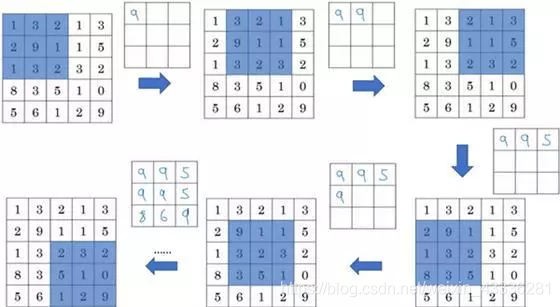
\includegraphics[width=0.9\textwidth]{pooling_1}
        \caption{最大值池化-前向传播 \cite{RN5}}
        \label{fig:11}
    \end{figure}

    \subsection{均值池化}
    
    ​ 在前向传播过程中,计算图像区域中的均值作为该区域池化后的值;在反向传播过程中,梯度特征分均配到各个位置。前向与反向传播的图示如图\ref{fig:12}与\ref{fig:13}所示。
    
    \begin{figure}[!htbp]
        \centering
        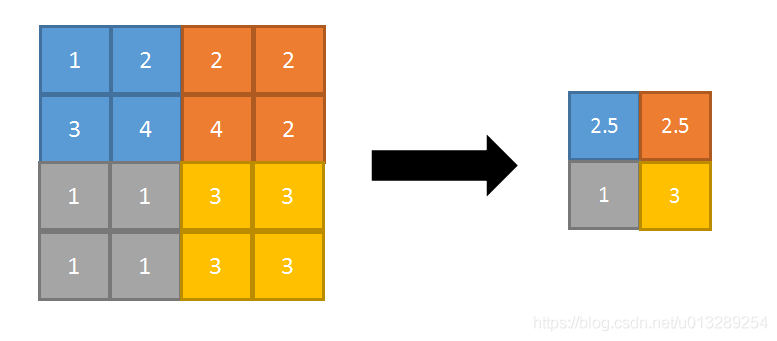
\includegraphics[width=0.9\textwidth]{pooling_2}
        \caption{均值池化-前向传播\cite{RN6}}
        \label{fig:12}
    \end{figure}
    \begin{figure}[!htbp]
        \centering
        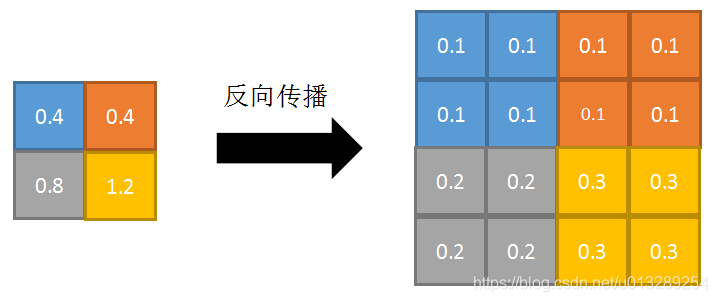
\includegraphics[width=0.9\textwidth]{pooling_3}
        \caption{均值池化-反向传播}
        \label{fig:13}
    \end{figure}

    在实际应用中,均值池化往往以全局均值池化的形式出现。常见于SE模块以及分类模块中。极少见于作为下采样模块用于分类网络中。
    
    均值池化的优点在于可以\uwave{减小估计均值的偏移,提升模型的鲁棒性}。
    
    \subsection{随机池化}
    
    ​ 随机池化是ICLR2013的一篇论文Stochastic Pooling,提出的一种池化策略,另有CVPR2017的一篇论文S3Pool提出一种随机位置池化策略。
    
    ​ 随机池化的方法非常简单,只需对特征区域元素按照其概率值大小随机选择,元素值大的被选中的概率也大。随机位置池化则集成了随机池化与最大值池化两者。示例如图\ref{fig:14}所示。
    
    \begin{figure}[!htbp]
        \centering
        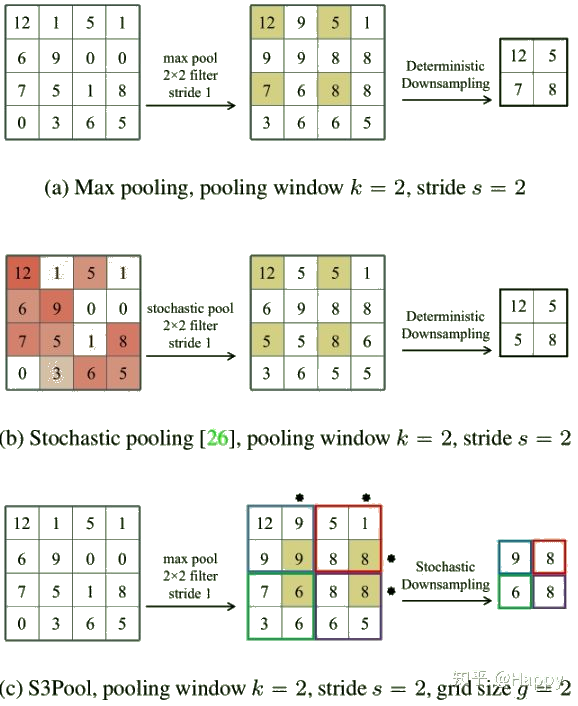
\includegraphics[width=0.7\textwidth]{pooling_4}
        \caption{\textit{Stochastic Pooling} and \textit{S3Pool}}
        \label{fig:14}
    \end{figure}

    \subsection{中值池化}
    
    中值池化是参考图像处理中的中值滤波而引申的一种池化方式。在目前CNN架构中极为少见,仅发现一篇论文:基于卷积神经网络和中值池化的人脸识别\cite{RN7},不确定是否为水文。
    
    ​在前向与反向传播过程中,中值池化类似于最大值池化,故不再赘述。
    
    ​中值池化同样具有学习边缘和纹理结构的特性,同时具有抗噪性。
    
    \subsection{分数阶最大值池化}
    
    ​ 分数阶最大值池化(Fractional Max Pooling)见诸于arXiv\cite{RN8}。本文查阅Pytorch代码时发现的,先前未曾了解过,也未曾用过。感兴趣者可以参见原文或者用pytorch代码试玩几把,这里提供一个pytorch试玩deme。
    

    \begin{lstlisting}
        import torch
        import torch.nn as nn
        inputs = torch.rand(20, 16, 50, 32)
        fmp = nn.FractionalMaxPool2d(3, output_ratio=(0.8, 0.8))
        output = fmp(inputs)
        print(output.size())
        # 此时output的尺寸为:20X16X40X25.
    \end{lstlisting}

    \subsection{组合池化}
    
    ​组合池化则是同时利用最大值池化与均值池化两种的优势而引申的一种池化策略。常见组合策略有两种:Cat与Add。其代码描述如下:
    
    \begin{lstlisting}
        def add_avgmax_pool2d(x, output_size=1):
        x_avg = F.adaptive_avg_pool2d(x, output_size)
        x_max = F.adaptive_max_pool2d(x, output_size)
        return 0.5 * (x_avg + x_max)
        
        def cat_avgmax_pool2d(x, output_size=1):
        x_avg = F.adaptive_avg_pool2d(x, output_size)
        x_max = F.adaptive_max_pool2d(x, output_size)
        return torch.cat([x_avg, x_max], 1)
    \end{lstlisting}